\documentclass[11pt]{scrartcl}
\usepackage[sexy]{../../../evan}
\usepackage{graphicx}
\usepackage{float}

\definecolor{dg}{RGB}{2,101,15}
\newtheoremstyle{dotlessP}{}{}{}{}{\color{dg}\bfseries}{}{ }{}
\theoremstyle{dotlessP}
\newtheorem{property}[theorem]{Property}

\newtheoremstyle{dotlessN}{}{}{}{}{\color{teal}\bfseries}{}{ }{}
\theoremstyle{dotlessN}
\newtheorem{notation}[theorem]{Notation}
% Shortcuts
\DeclarePairedDelimiter\ceil{\lceil}{\rceil} % ceil function

\DeclarePairedDelimiter\paren{(}{)} % parenthesis

\newcommand{\df}{\displaystyle\frac} % displaystyle fraction
\newcommand{\qeq}{\overset{?}{=}} % questionable equality

\newcommand{\Mod}[1]{\;\mathrm{mod}\; #1} % modulo operator

\newcommand{\comp}{\circ} % composition

% Text Modifiers
\newcommand{\tbf}{\textbf}
\newcommand{\tit}{\textit}

% Sets
\DeclarePairedDelimiter\set{\{}{\}}
\newcommand{\unite}{\cup}
\newcommand{\inter}{\cap}

\newcommand{\reals}{\mathbb{R}} % real numbers: textbook is Z^+ and 0
\newcommand{\ints}{\mathbb{Z}}
\newcommand{\nats}{\mathbb{N}}
\newcommand{\complex}{\mathbb{C}}
\newcommand{\tots}{\mathbb{Q}}

\newcommand{\degree}{^\circ}

% Counting
\newcommand\perm[2][^n]{\prescript{#1\mkern-2.5mu}{}P_{#2}}
\newcommand\comb[2][^n]{\prescript{#1\mkern-0.5mu}{}C_{#2}}

% Relations
\newcommand{\rel}{\mathcal{R}} % relation

\setlength\parindent{0pt}

% Directed Graphs
\usetikzlibrary{arrows}
\tikzset{vertex/.style = {shape=circle,draw,minimum size=2em}}
\tikzset{svertex/.style = {shape=circle,draw,minimum size=.05em,font=\tiny}}
\tikzset{edge/.style = {->,> = latex'}}
\tikzset{dedge/.style = {-> = latex'}}
\tikzset{dot/.style={inner sep=1.5pt,circle,draw,fill}}


% Contradiction
\newcommand{\contradiction}{{\hbox{%
    \setbox0=\hbox{$\mkern-3mu\times\mkern-3mu$}%
    \setbox1=\hbox to0pt{\hss$\times$\hss}%
    \copy0\raisebox{0.5\wd0}{\copy1}\raisebox{-0.5\wd0}{\box1}\box0
}}}

\newcommand{\xxhash}[2]{\rotatebox[origin=c]{#2}{$#1\parallel$}}

\title{CS 120: Intro to Algorithms and their Limitations}
\subtitle{PSet 4}
\author{Denny Cao}
\date{\today}
%++++++++++++++++++++++++++++++++++++++++
% title stuff
\usepackage{titling}
\renewcommand\maketitlehooka{\null\mbox{}\vfill}
\renewcommand\maketitlehookd{\vfill\null}
\makeatletter
\renewcommand{\maketitle}{\bgroup\setlength{\parindent}{0pt}
	\begin{flushleft}
		\large\textbf{\@title} \\ \vskip 0.2cm
		\begingroup
		\fontsize{14pt}{12pt}\selectfont
		\title
		\\
		Problem Set 4
		\endgroup \vskip 0.3cm
		Due: October 18, 2023 11:59pm \hfill\rlap{}\textbf{Denny Cao} \\ \vskip 0.1cm
		\hrulefill
	\end{flushleft}\egroup
}
\makeatother

\renewcommand{\theques}{\thesection.\alph{ques}} % Change subtheo counter for alpha output
\declaretheorem[style=basehead,name=Answer,sibling=theorem]{ans}
\renewcommand{\theans}{\thesection.\alph{ans}}
\begin{document}
\maketitle
\pagestyle{plain}
\textbf{Collaborators:}

\textbf{No. of late days used on previous psets:} 1

\textbf{No. of late days used after including this pset:} 2
\section{Randomized Algorithms in Practice}
\begin{enumerate}[(a)]
	\item In \texttt{ps\_4.py}.
	\item The table below depicts corresponding values of $k$ for each $n$:
		\begin{figure}[H]
		\centering
		\begin{tabular}{c|c}
			$n$ & $k^*_n$ \\
			\hline
			1024 & 29 \\
			2048 & 29 \\
			4096 & 31 \\
			8192 & 33 \\
			16384 & 34 \\
			32768 & 36
		\end{tabular}
	\end{figure}
	From running the experiment for $25 \leq k \leq 39$, we obtain the following graphs for each $n$:
	\begin{figure}[H]
		\centering
	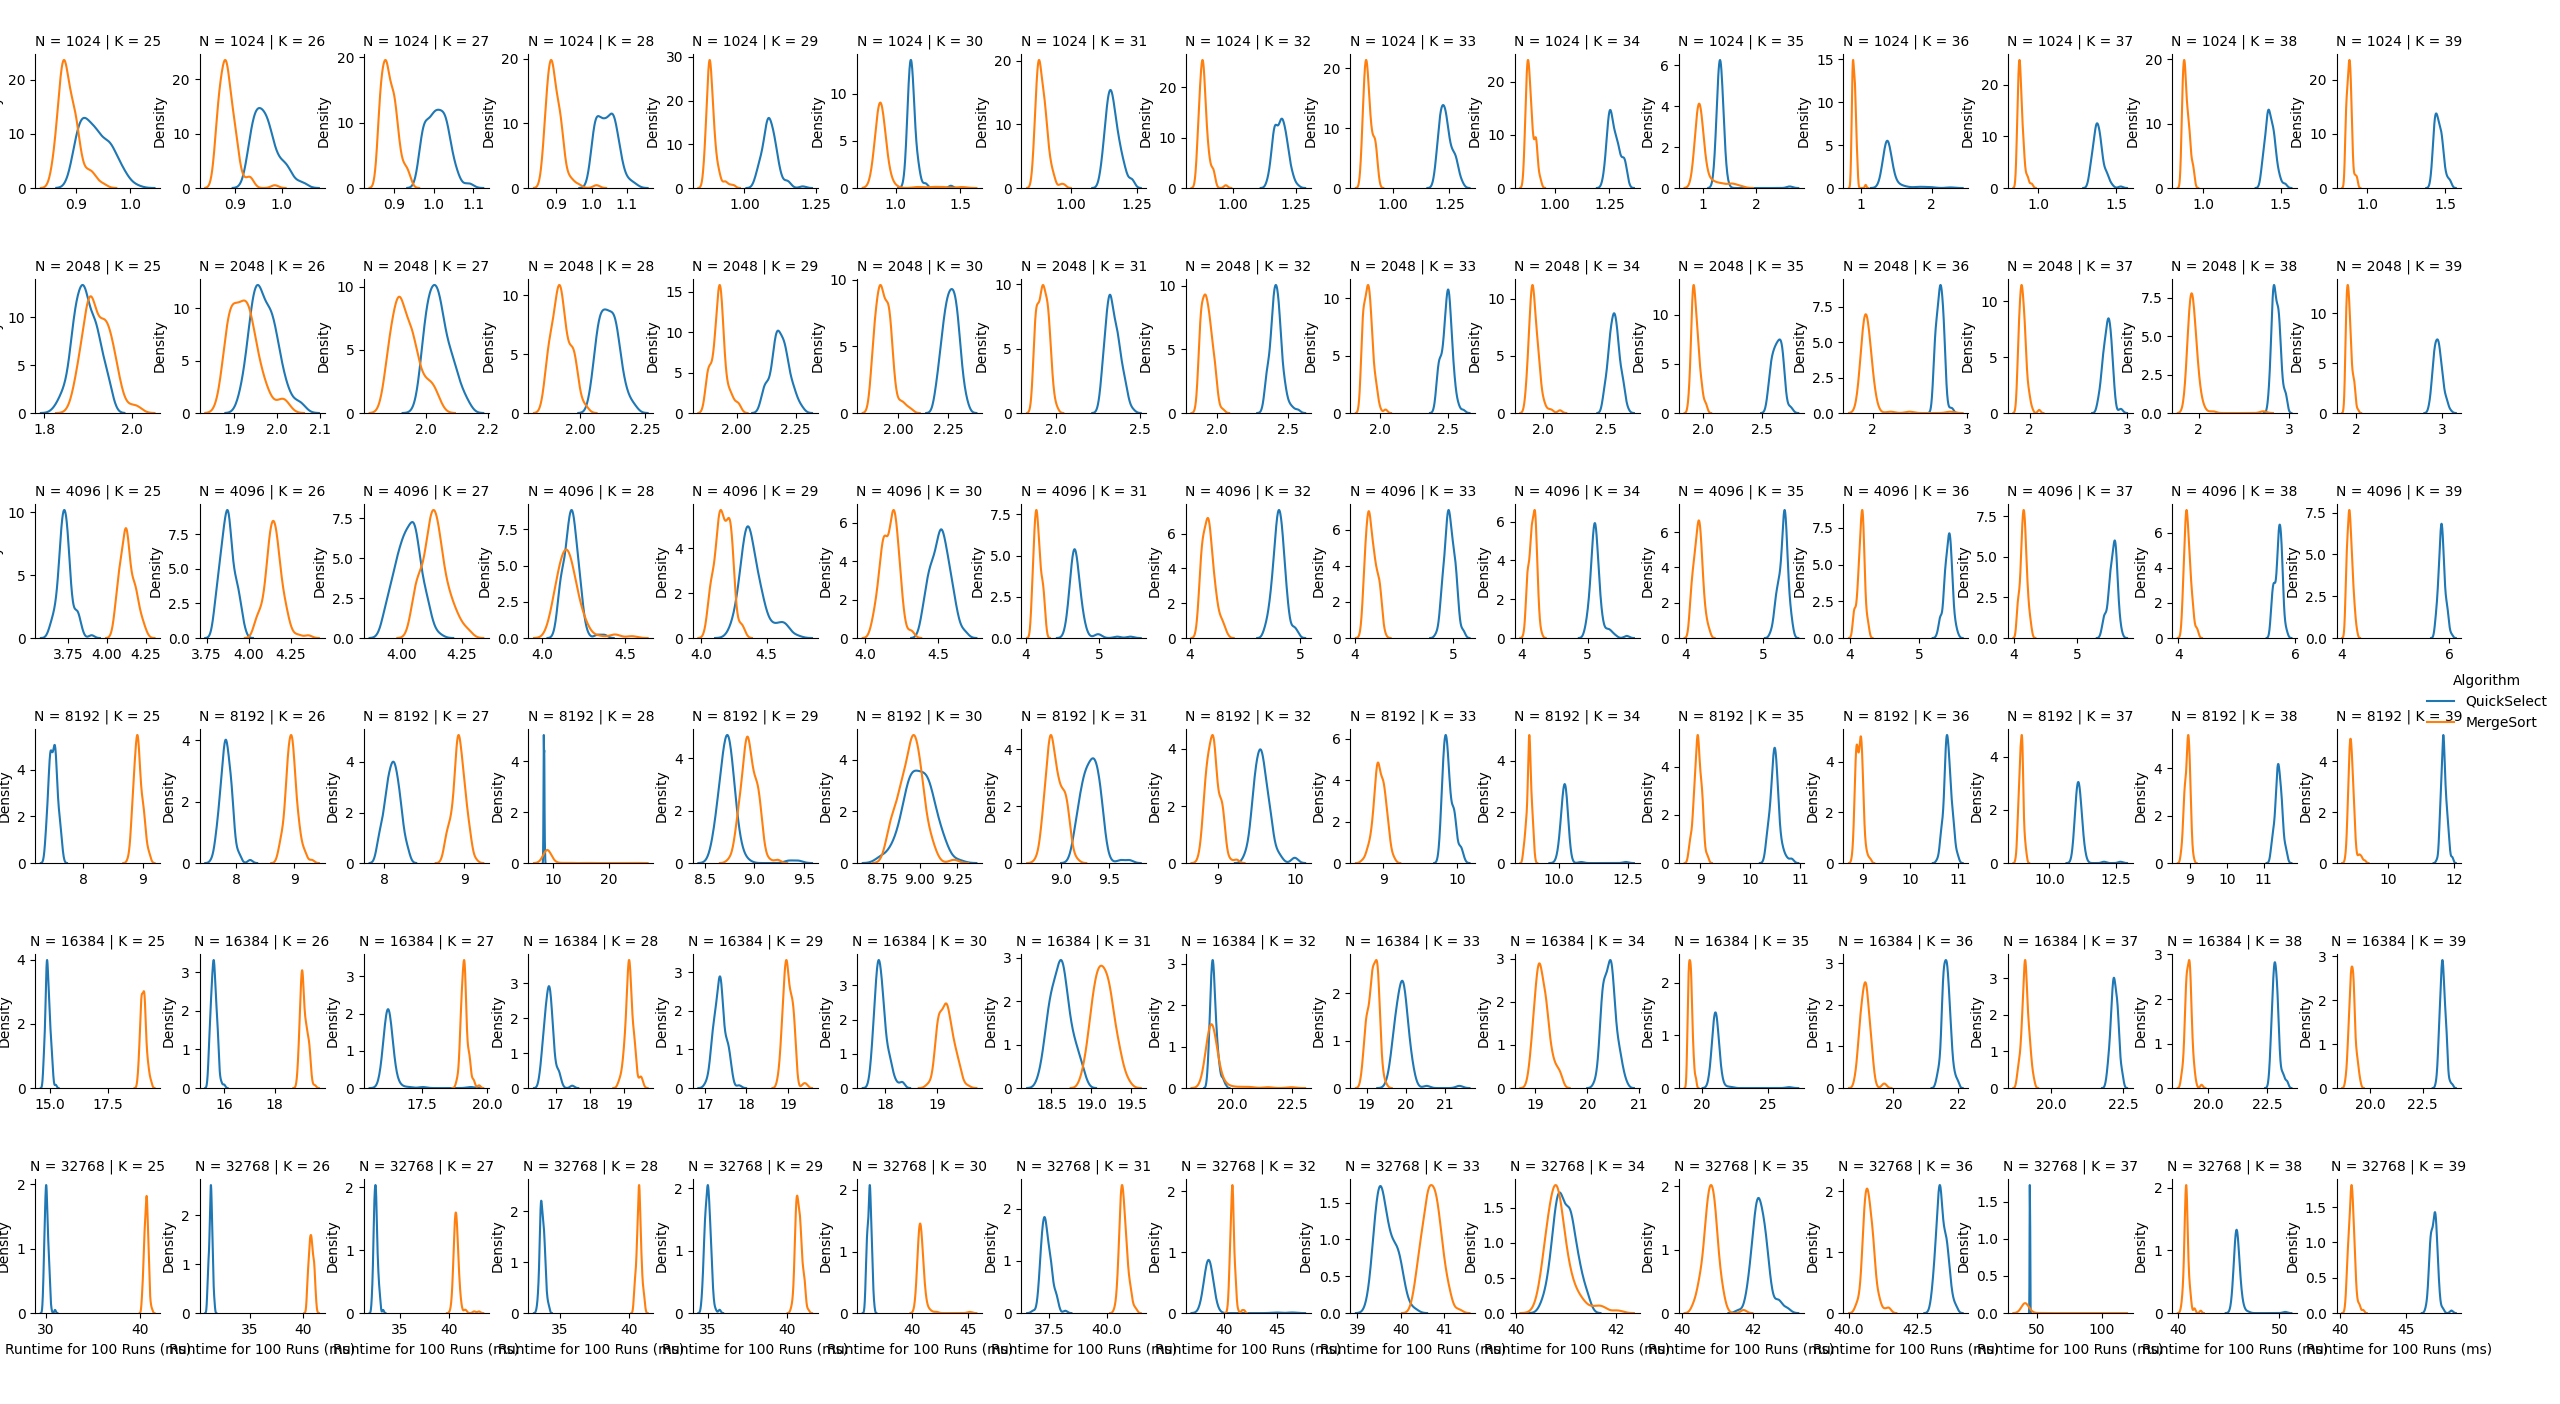
\includegraphics[width=\textwidth]{Figure_1.png}
	\end{figure}
	We select the least value $k$ for each $n$ when the distribution of runtimes for \texttt{MergeSortSelect} is less than the distribution of runtimes for \texttt{QuickSelect}, as this would imply that, for that chosen $k$, \texttt{MergeSortSelect} is faster than \texttt{QuickSelect}, it is the first $k$ such that \texttt{MergeSortSelect} is the faster algorithm on average than \texttt{QuickSelect}.
\item A functional form for $k_n^*$ could be the following:
	\[
	k^*(n) = \log_2 n + 20
	\] 
\item \
	\begin{figure}[H]
		\centering
		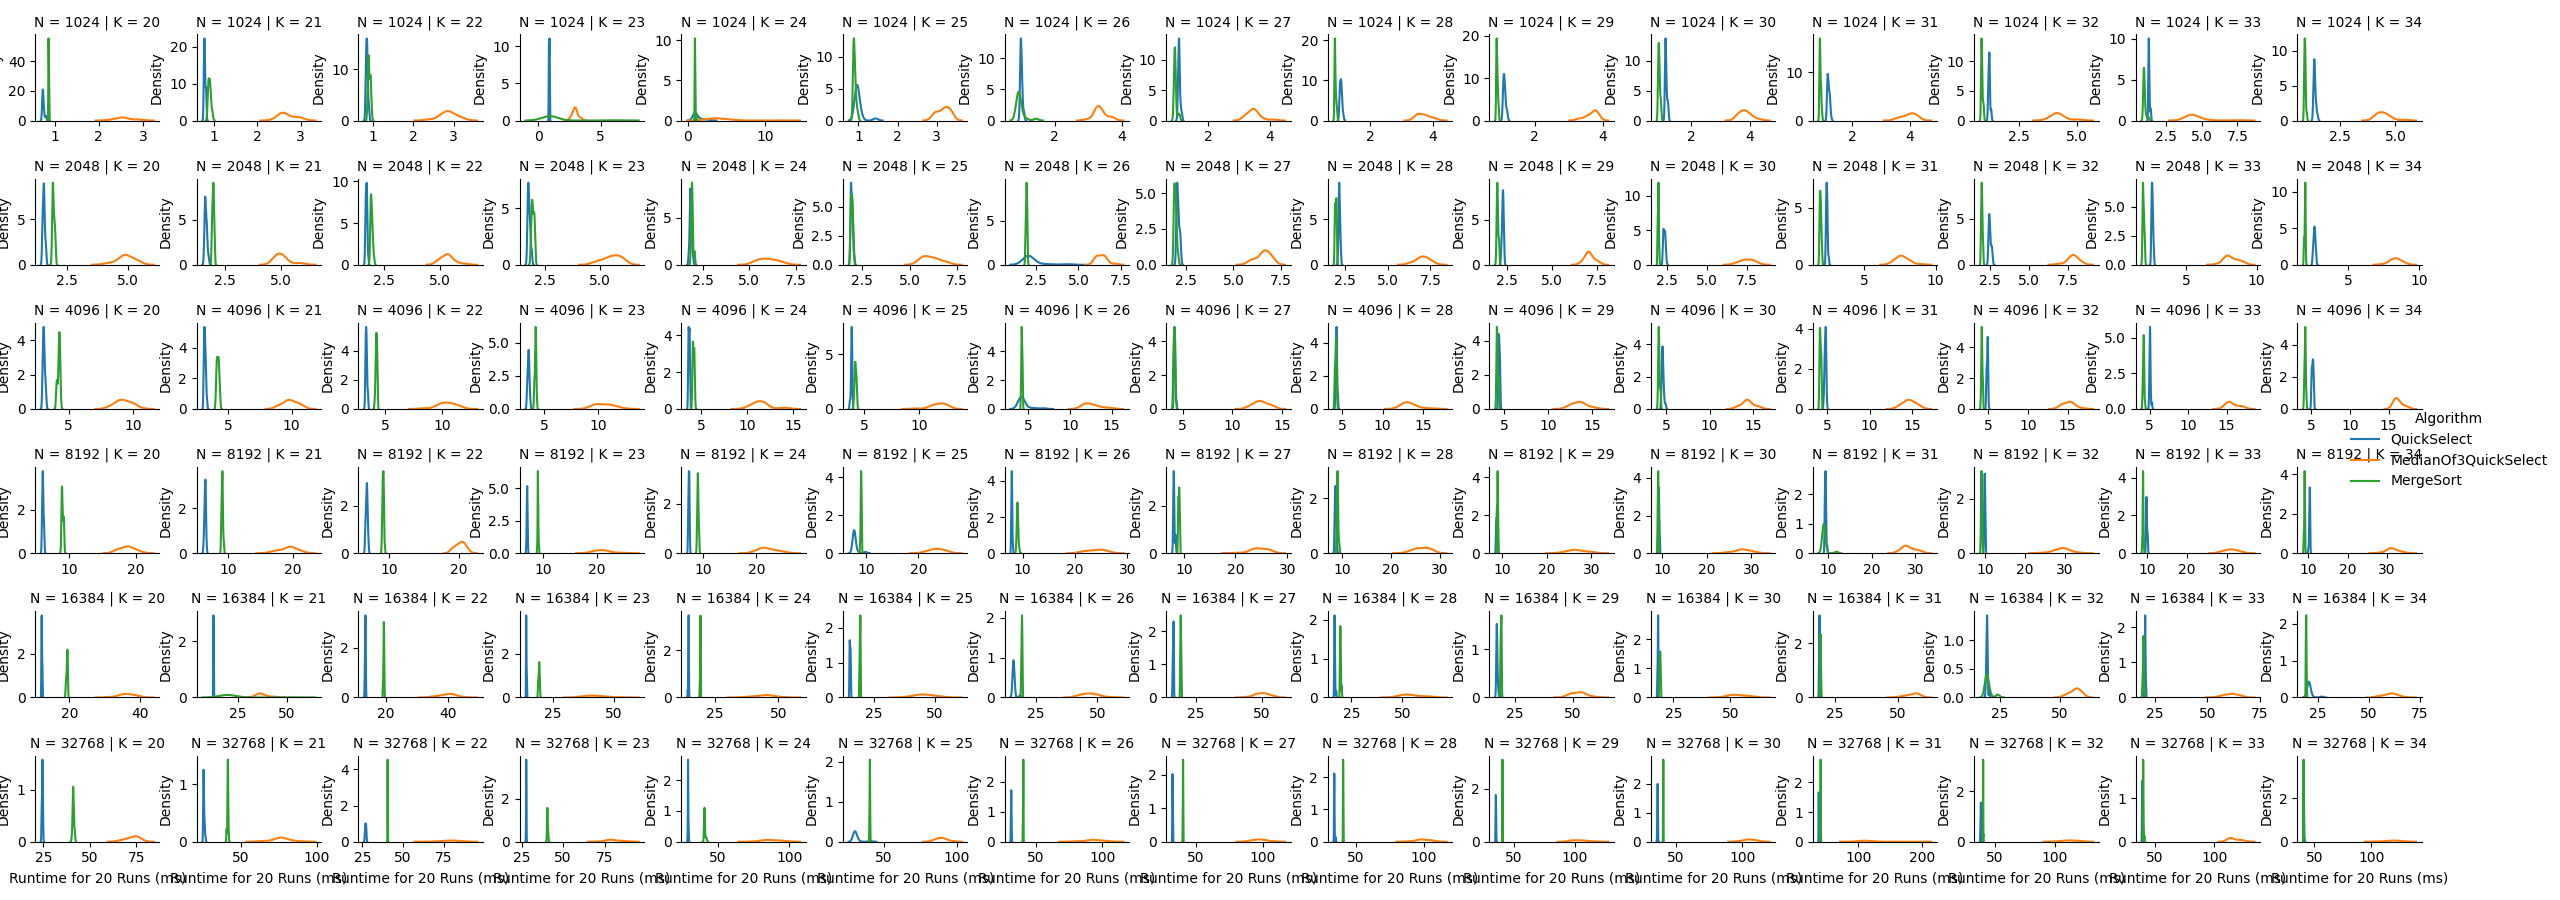
\includegraphics[width=\textwidth]{Figure_2.png}
	\end{figure}
	The expected result is that, by selecting the pivot position with less randomness, we can have more ``even'' splits of the array, decreasing the chance that \texttt{QuickSelect} reaches the $O(n^2)$ time.  
\end{enumerate}
\section{Dictionaries and Hash Tables}
\begin{claim*}
	\texttt{DuplicateSearch} can be solved by a Las Vegas algorithm with expected runtime $O(n)$ using a dictionary data structure.
\end{claim*}
\begin{proof}
	We first describe the Las Vegas algorithm:
	\begin{enumerate}
		\item \texttt{Preprocess($\reals$,$m$)}: Initialize an array $A$ of size $m$, where $m = \Theta(n)$. Choose a random hash function $h: \reals \to [m]$.
		\item We will now loop through all elements $(K,V)$ of the input array and do the following:
			\begin{enumerate}
				\item \texttt{Search($K$)}: Walk through the linked list $A[h(K)]$. If search returns an element, we return $K$. If search returns $\perp$, continue.
				\item \texttt{Insert($K,V$)}: Insert $(K,V)$ at the head of linked list slot $A[h(K)]$.
			\end{enumerate}
		\item If the loop is completed, return $\perp$.
	\end{enumerate}
	We now want to prove our algorithm:
	\begin{enumerate}
		\item has the desired runtime and
		\item is correct.
	\end{enumerate}
	\begin{itemize}
		\item Initializing an array of size  $O(n)$ will take $O(n)$ time. For each element $(K,V)$ in the input array, \texttt{Search($K$)} will take an expected time of $O(1)$, as \texttt{Search($K$)} takes $O(1 + \frac{n}{m})$ and $m = \Theta(n) \implies m = \Omega(n)$. $\texttt{Insert($K,V$)}$ will also take $O(1)$, as we simply insert the element at the head of the linked list at $A[h(K)]$. At the worst case, we iterate through all elements of the input array, and, as we take an expected time of $O(1)$ time for $n$ elements, it will expectedly take $O(n)$ time. Thus, in total, the expected run time is the time for preprocessing and the expected time it takes for the loop: $O(n) + O(n) = O(n)$.
		\item Before inserting a key value pair $(K,V)$, we run \texttt{Search($K$)} which will only return if the dictionary contains a key value pair $(K,V^*)$. The only values in the dictionary are key value pairs from the input that were inserted when $\texttt{Search($K$)}$ returns $\perp$; $\texttt{Search($K$)}$ will only return $K$, causing the algorithm to return $K$ when there exists a duplicate, and the loop will complete only if for all $(K,V)$ in the input array, $\texttt{Search($K$)}$ returns $\perp$ prior to inserting, causing the algorithm to return  $\perp$, meaning there is no duplicate present.
	\end{itemize}
	We have shown that there exists a Las Vegas algorithm with expected runtime $O(n)$ using a dictionary structure and that the algorithm is correct.
\end{proof}
\section{Rotating Walks}
\begin{enumerate}[(a)]
	\item \begin{proof}
	We first describe the reduction algorithm:
	\begin{enumerate}
		\item \texttt{Preprocess}: We preprocess a new digraph $G'$ as follows:
			\begin{itemize}
				\item Define the vertex set $V'$ of $G'$ to be the set of pairs $(v, j)$, where $v \in V$ is a vertex from the original digraph, and $j \in [k]$	
				\item For each pair of vertices $(v, j)$ and $(w, j+1 \bmod k)$ in $V'$, if there is an edge $(v, w)$ in $E_{j+1 \bmod k}$, then add an edge from $(v, j)$ to $(w, j+1 \bmod k)$ in $E'$, the edge set of $G'$.
			\end{itemize}
		\item Make an oracle call \texttt{SingleSourceShortestPaths($G',(s, 0)$)}.
		\item \texttt{Postprocess}: As the oracle returns an array of shortest paths from $s$ to all other vertices  $v \in V'$, we iterate to find the shortest path amongst $(t,j) \forall j \in [k]$; we find:
			\[
				\texttt{dist}_{G'}((s,0), (t,x)) \leq \texttt{dist}_{G'}((s,0), (t,j)) \forall j \in [k], x \in [k]
			\] 
		\item Return the path from $(s,0)$ to  $(t,x)$.
	\end{enumerate}
	We now want to prove our algorithm:
	\begin{enumerate}
		\item has the desired runtime and
		\item is correct.
	\end{enumerate}
	\begin{itemize}
		\item Preprocessing $G'$ takes $O(kn)$, as we iterate through all $n$ vertices for each of the $k$ diagraphs. \texttt{SingleSourceShortestPaths} can be solved in $O(n + m)$, where $n$ is the number of vertices and $m$ is the number of edges. As we call the oracle on  $G'$ which has a vertex set $V' = \set*{(v_0, 0), \dots, (v_0, k-1), \dots, (v_{n-1}, 0), (v_{n-1}, k-1)}$ and thus $|V| = kn$ and an edge set $E'$ where $|E'| = |E_0| + |E_1| + \dots + |E_{k-1}|$, $|E'| = m_0 + m_1 + \dots + m_{k-1}$, \texttt{SingleSourceShortestPaths} on $G'$ can be solved in time $O(|V'| + |E'|) = O(kn + m_0 + m_1 + \dots + m_n)$. The time it takes during postprocessing to iterate through all shortest paths to find the shortest path from $(s,0)$ to  $(t,x)$ takes  $O(kn)$. Thus, the total runtime is  $O(kn) + O(kn + m_0 + m_1 + \dots + m_{k-1}) + O(kn) = O(kn + m_0 + m_1 + \dots + m_{k-1})$. 
		\item As each edge in  $G'$ is of the form $((v_i, j), (v_t, j+1 \mod k))$, each edge is a rotation from  $G_j$ to $G_{j+1 \mod k}$. We can thus use \texttt{SingleSourceShortestPaths} to find the shortest path from any vertex to another formed by any rotated path.
	\end{itemize}
	We have shown that the problem of \texttt{ShortestRotatingWalk} from $s$ to $t$ with respect to $G_0, \dots, G_{k-1}$ can be reduced to \texttt{SingleSourceShorestPaths} with the desired runtime and that the algorithm is correct.
\end{proof}

\item \
	\begin{figure}[H]
		\centering
		\begin{tabular}{c|c|c}
			$d$ & Frontier $F_d$ & Predecessor Relationships \\
			\hline
			0 & $\set*{(a,0)}$ & \\
			1 & $\set*{(b,0)}$ &  $((a,0), (b,0))$ \\
			2 & $\set*{(d,1), (e,1)}$ &  $((b,0),(d,1)),((b,0),(e,1))$ \\
			3 & $\set*{(d,0),(g,0)}$ &  $((e,1),(d,0)),((e,1),(g,0))$ \\
			4 & $\set*{(f,1),(c,1)}$ &  $((d,0),(c,1)), ((d,0), (f,1), ((g,0),(f,1))$
		\end{tabular}
	\end{figure}
\item
\begin{proof}
	Let vertices be denoted by $v_{ij}$ where  $i$ is the row and $j$ is the column. Let $G_0, G_1, G_2$ denote the graphs of Player 0, Player 1, and Player 2 respectively and the possible positions they can move.
	\begin{itemize}
		\item $G_0$, since Player 0 can move like a chess rook, Player 0 can move from a vertex $v_{ab}$ to a vertex  $v_{a,x}$ or $v_{x,b}$ where  $0 \leq x \leq n$. Each vertex can move to $2n-2$ other vertices, and as there are $n^2$ vertices,$|E_0| = n^2(2n-2) = O(n^3)$.
		\item $G_1$, since Player 1 can move like a chess bishop and the greatest amount of outward edges for a vertex is $2n-2$, we know  $|E_1| \leq n^2(2n-2) = O(n^3)$.
		\item $G_2$, since Player 2 can move like a knight which has at most 8 outward edges for a vertex, $|E_2| \leq 8n^2 = O(n^2)$.
	\end{itemize}
	We now call the oracle \texttt{ShortestRotatingPaths} with the graphs $G_0, G_1, G_2$ and start position $s$ and desired position $t$, which will have runtime $O(|V| + |E|)$. As  $|V| = n^2$ and  $|E| = |E_0| + |E_1| + |E_2| = O(n^3) + O(n^3) + O(n^2) = O(n^3)$, the runtime will be  $O(n^2 + n^3) = O(n^3)$, as desired.
\end{proof}
\end{enumerate}
\end{document}
